\documentclass[12pt,a4paper]{article}

\usepackage{anyfontsize}
\usepackage{graphicx}

%package for list formatting (ordered) if we add [a.]
\usepackage{enumerate}
%package for graphics or include images
\usepackage{graphicx}
\usepackage{float} %to place image forcefully there

\usepackage{subcaption,caption}
\usepackage[hidelinks]{hyperref}

%for times new roman font
\usepackage{times,mathptmx}


%package for margins
\usepackage[outer=1.25in,inner=1.5in,top=1in,bottom=1in,headheight=0.5in,footskip=0.5in]{geometry}
%better to use outer and inner beacause while printing book then right and left margin will not be good , So, inner margin 


\begin{document}
	\pagenumbering{roman}
	
	
\begin{titlepage}
	
	\newcommand{\HRule}{\rule{\linewidth}{0.3mm}}
	\centering
	\vfill
	
\includegraphics[width=50mm]{images/tu.jpg}\\[0.75cm]
	\textsc{\Large \bfseries  TRIBHUVAN UNIVERSITY}\\[0.25cm] % Name of your university/college
	\textsc{\Large \bfseries INSTITUTE OF ENGINEERING}\\[0.25cm]
	\textsc{\Large \bfseries  PULCHOWK CAMPUS}\\
	\vfill
	\large {A PROJECT REPORT ON }\\
	\Large \textbf{Tetris: The Classic Puzzle Game}
	\vfill
	%\large \textbf{Subject code} \\[0.2cm]
%	\bfseries
	\large
		\textbf{Submitted by:}\\
	AASHISH KARKI (078BCT004)\\
	ANUP ARYAL (078BCT015)\\
	APIL CHAUDHARY (078BCT017)\\[0.5cm]
	\vfill
		\textbf{SUBMITTED TO:}\\
	DEPARTMENT OF ELECTRONICS AND COMPUTER ENGINEERING\\
	IOE, Pulchowk Campus\\
	Kathmandu Nepal
	\\
	\vfill
	{\large \today}
	\vfill
\end{titlepage}

	
  	
  	
  	\newpage
\pagenumbering{arabic}
\section{ACKNOWLEDGEMENT}


We express our sincere gratitude to our teachers(Mr. Daya Sagar Baral, Mr. Aman Shakya and Mr. Rajad Shakya) who suggested building this game for sharpening our Object Oriented Programming skills and logic building capabilities.

\vspace{5mm}
Our special thanks goes to our lecturer, Daya Sagar Baral, for his guidelines, suggestions, and instructions, which have served as a contributor towards the inception of this project.

\vspace{5mm}
We sincerely thank the Department of Electronics and Computer Engineering, Pulchowk Campus, for giving us an opportunity to work on this project to expand our knowledge of Object Oriented Programming and working in a team.

  
  	
  	%\newpage
  	%{
  	%	\setlength{\parskip}{0em}
  	%	\renewcommand\contentsname{TABLE OF CONTENTS}\\[0.5cm] % This will change heading text
  	%	\tableofcontents 
  	   % \addcontentsline{toc}{section}{TABLE OF CONTENTS}
  	%}
  	
  	
  	
  	
  	\newpage
\pagenumbering{arabic}
\section{INTRODUCTION}
\hspace{5mm}Tetris, an iconic and enduring puzzle game, has captured the hearts of gamers around the world since its inception in 1984. Created by Russian game designer Alexey Pajitnov, Tetris challenges players with a deceptively simple objective: fitting different-shaped blocks, known as tetrominoes, together to form complete lines. Yet, beneath its straightforward premise lies an addictive and exhilarating experience that has stood the test of time.\\

\textbf{Gameplay :} \\

\textbf{Tetrominoes:} The game consists of various tetrominoes, each made up of four connected squares arranged in different shapes. The seven tetrominoes are: I, J, L, O, S, T, and Z.\\

\textbf{Falling Blocks: }Tetrominoes fall from the top of the playing area one at a time. You have the ability to move and rotate the tetrominoes as they descend.\\

\textbf{Movement and Rotation:} You can move the falling tetrominoes horizontally (left or right) using the arrow keys or buttons. You can also rotate them clockwise or counterclockwise to fit them into available spaces using the up arrow key or designated rotation buttons.\\

\textbf{Clearing Lines:} The primary goal is to create complete horizontal lines by filling all the spaces within a row. When a line is entirely filled, it clears from the screen, and you earn points.\\

\textbf{Scoring:} The more lines you clear at once, the higher the points you earn. Clearing multiple lines simultaneously is known as a "Tetris" and yields the highest points.\\

\textbf{Leveling Up:} As you accumulate points or clear a certain number of lines, you advance to higher levels. With each level, the tetrominoes fall faster, increasing the game's difficulty.\\

\textbf{Game Over:} The game ends when the stack of falling tetrominoes reaches the top of the playing area. If you can't clear lines fast enough, the stack will reach the top, and the game will be over.\\

\textbf{Controls:}\vspace{5mm}\\
The controls for Tetris are usually straightforward:\\
\textbf{Left Arrow: }Move tetromino left\\
\textbf{Right Arrow: }Move tetromino right\\
\textbf{Down Arrow: }Accelerate the fall of the tetromino\\
\textbf{Up Arrow: }Rotate tetromino clockwise or counterclockwise\\


  	\newpage
\section{OBJECTIVES}
The objectives of building this game in C++ are listed below:


\begin{enumerate}
\item \textbf{Use Object-Oriented Programming (OOP):}
	\begin{itemize}
		\item Create classes for Tetrominoes, game board, and game logic.
		\item Organize code for easy maintenance and flexibility.
	\end{itemize}
	
\item \textbf{Explore C++ Features:}
\begin{itemize}
	\item Manage game data efficiently using vectors, pairs, maps and other containers in STL.
	\item Handle resources smartly to optimize performance.
\end{itemize}

\item \textbf{Graphics with SFML:}
\begin{itemize}
	\item Use SFML to draw Tetrominoes, game board, and animations.
	\item Respond to player input using SFML's event system.
\end{itemize}

\item \textbf{Reusable Code:}
\begin{itemize}
	\item Create header files for sharing code across the game.
\end{itemize}

\item \textbf{Implement Game Mechanics:}
\begin{itemize}
	\item Make Tetrominoes rotate, move, and detect collisions.
	\item Create a scoring system and difficulty levels.Create a scoring system and difficulty levels.Create a scoring system and difficulty levels.
\end{itemize}

\item \textbf{Add Sound Effects and Music:}
\begin{itemize}
	\item Integrate audio using SFML for a better gaming experience.
\end{itemize}

\item \textbf{Test and Debug:}
\begin{itemize}
	\item Thoroughly test the game to fix any issues.
	\item Use logs and debugging tools for troubleshooting.
\end{itemize}

\item \textbf{Team Collaboration:}
\begin{itemize}
	\item Communicate well within the team.
	\item Use Git for version control and collaboration.
\end{itemize}
\end{enumerate}
  		\newpage
	
\section{PROPOSED SYSTEM}
\subsection{DESCRIPTION}
\subsubsection{background}
THIS IS DESCRIPTION \\ \\
\pagebreak
\subsection{SYSTEM BLOCK DIAGRAM}
THIS IS SYSTEM BLOCK DIAGRAM

  		\newpage
\section{METHODOLOGY}
\hspace{5mm}This  project aimed to develop a Tetris game using Object-Oriented Programming principles and the SFML library for graphics. The project was implemented using the CLion Integrated Development Environment and utilized CMake for cross-platform build support. Version control and collaborative coding was facilitated through Git and GitHub.\\
For detailed history of development of this game,\\
Link to our GitHub Repository:\\
\textit{https://github.com/Aashish079/Tetris}\\



To ensure a structured and maintainable codebase, we have designed the class hierarchy for the game. Different classes are created by inheriting from the parent class State, to represent game objects such as the GamePlayState class, GameOverState class, HighScoreState tetrominoes, and FileManager. We have employed OOP concepts such as encapsulation, inheritance, and polymorphism to achieve modularity and code reusability in this project. The game logic is implemented within the GamePlayState class. Each class have private and public member variables and member functions that handle specific aspects of the game, such as moving and rotating tetrominoes, checking for line clears, and updating the score. The SFML library is utilized for rendering graphics and handling user input.\\

To ensure efficient functioning, smooth transistioning and good development experience we have used starter code of SFML named TheStateMachine which stores and renders different states such as MainMenuState, GameplayState and GameOverState.\\

To facilitate collaboration among team members, we utilized Git and GitHub for version control. We had total of 7 different branches for different features. Regular commits were performed to the repository and timely pull request were initiated from different branches into main branch. GitHub's issue tracking feature was also utilized to manage and prioritize tasks. Proper documentation was maintained to provide an overview of the project structure, class hierarchy, and function specifications..\\

We tried our best to take the most systematic and effiecient development \\approach throughout the development of this project.\\

  	
\section{PROJECT SCOPE}
\hspace{5mm}This project is a clone of the classic Tetris game created by Alexy Pajitnov in 1985. It will abide by standard rules and mechanics of the original tetris game with clean and user-friendly interface. It is developed to practice and learn Object Oriented Programming in the game development context.

  	\newpage
\section{PROJECT SCHEDULE}

\begin{figure}[H]
	\centering
	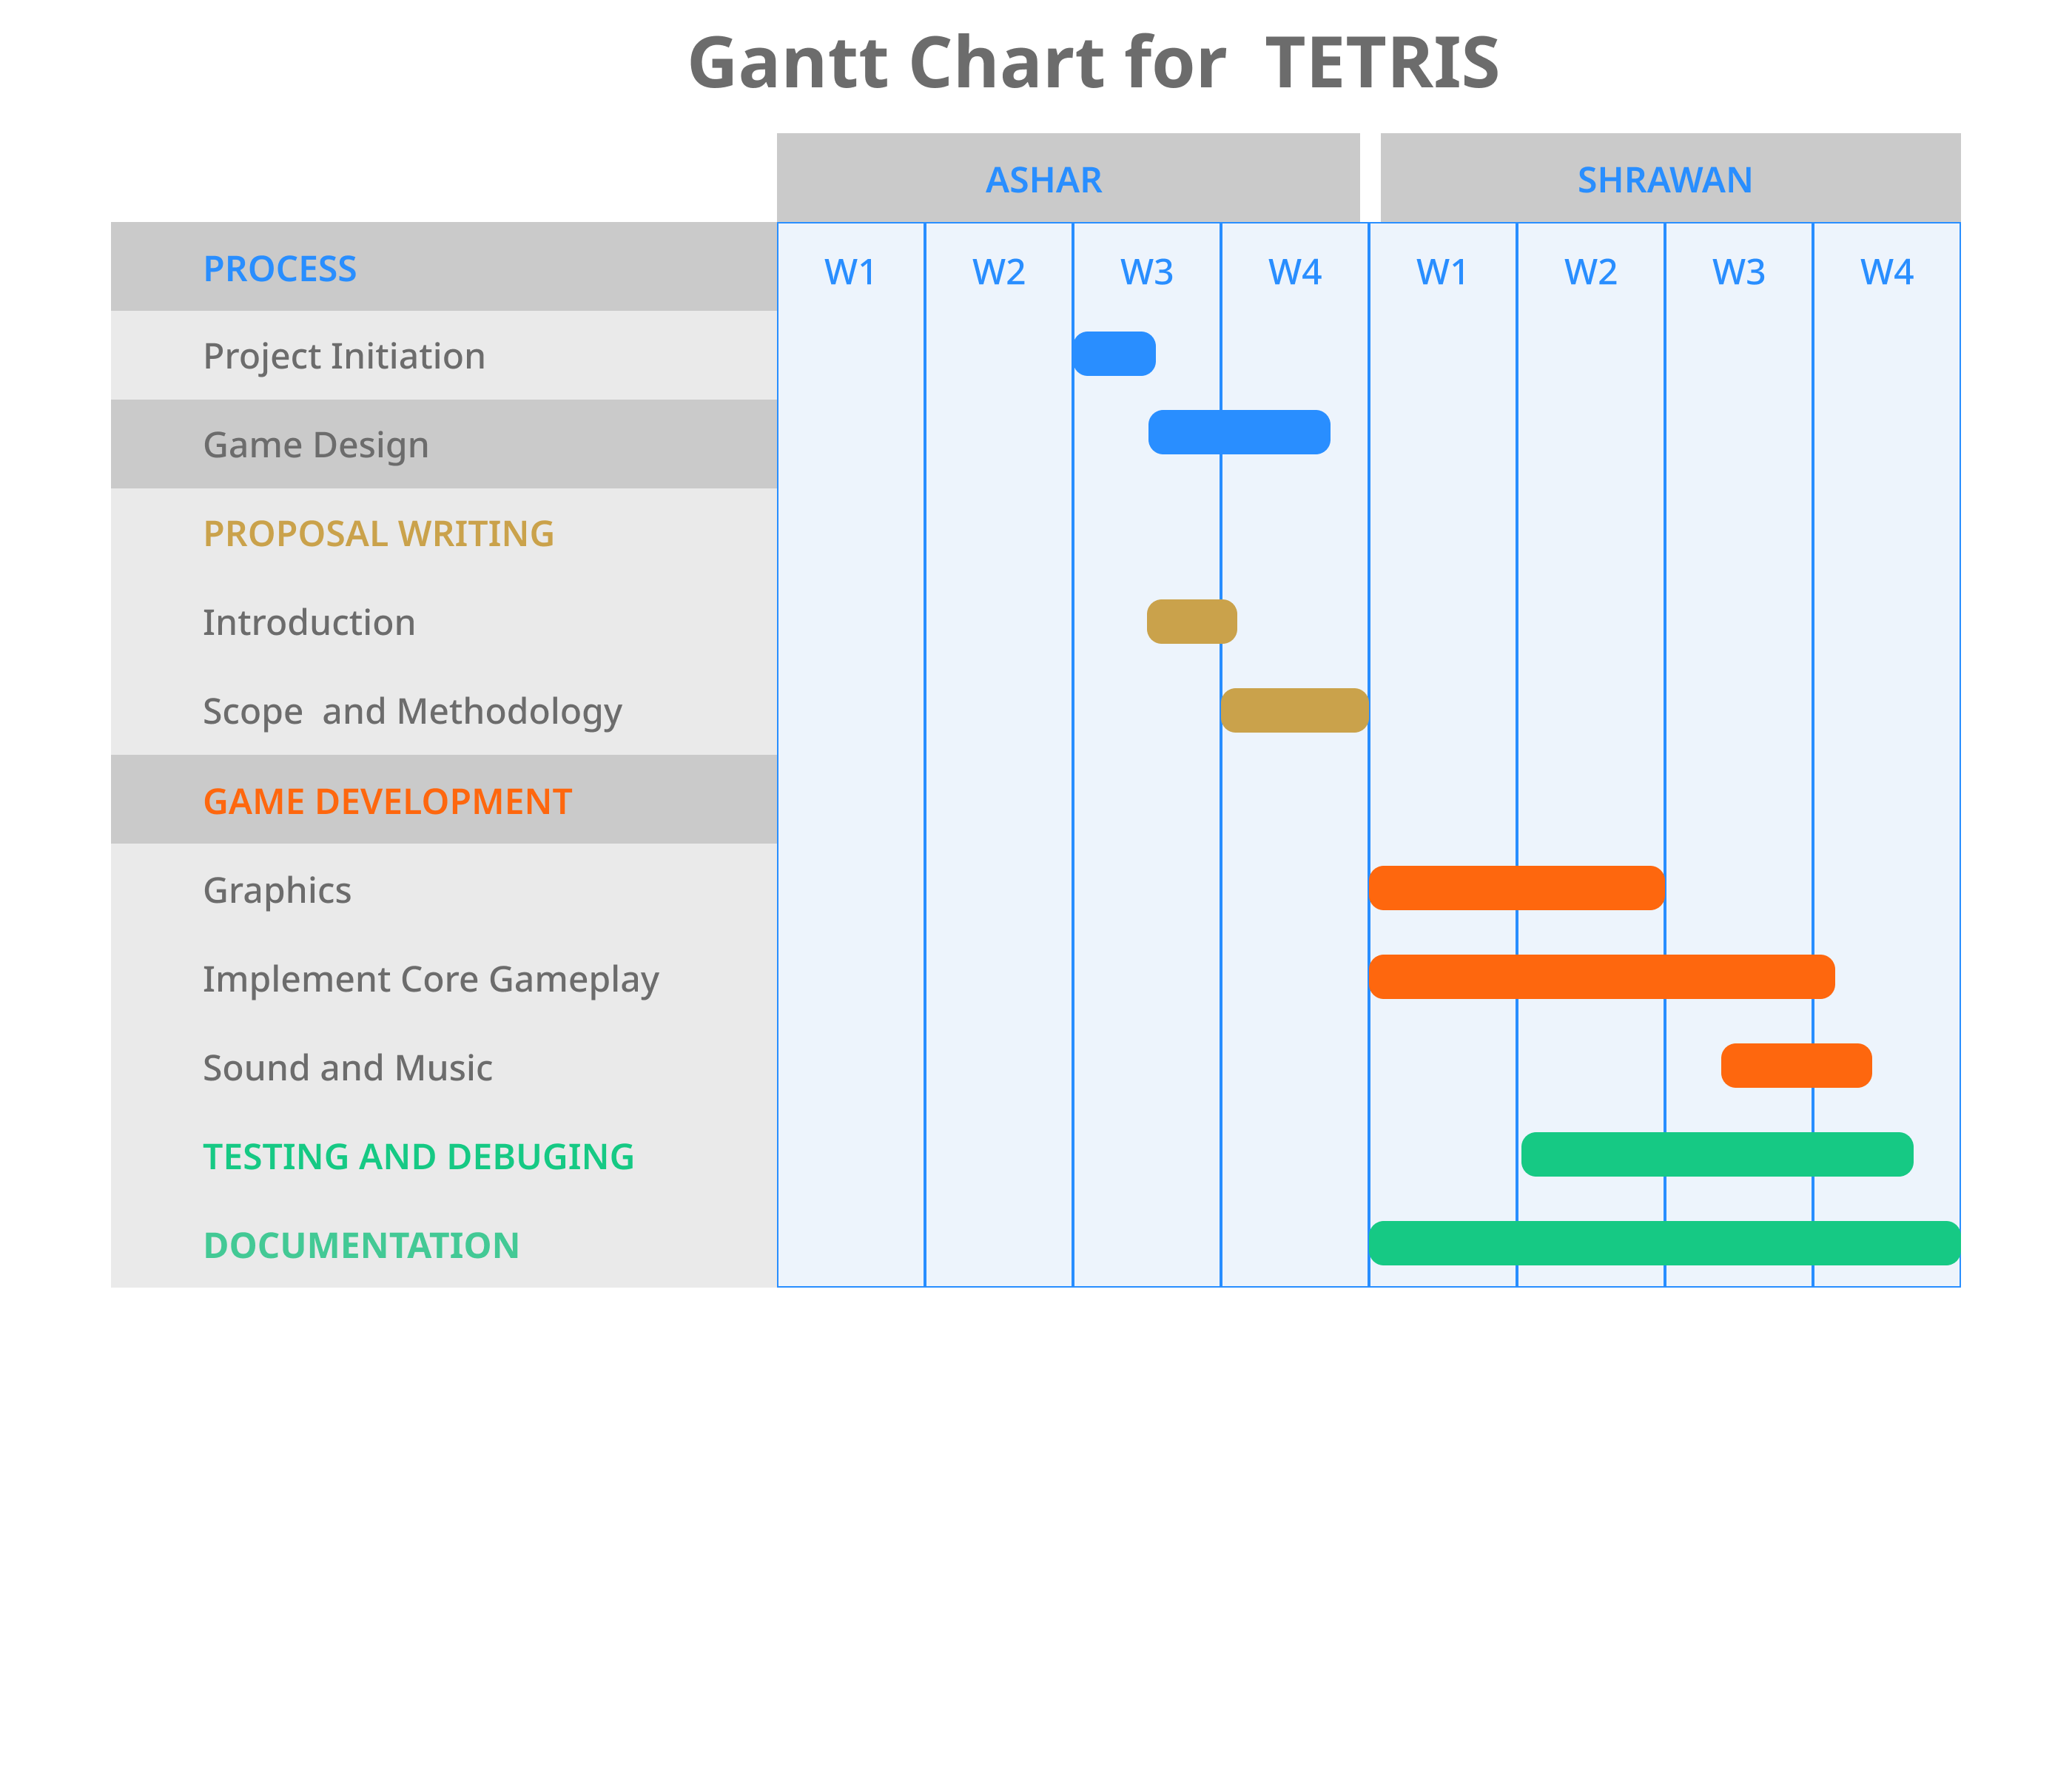
\includegraphics[width=\textwidth]{images/Gantt.png}
	\caption{Gantt Chart for OOP Project : TETRIS }
\end{figure}


  	
  	
  	
  	
  	
  
  
  
  
	
\end{document}


